\documentclass[]{book}
\usepackage{lmodern}
\usepackage{amssymb,amsmath}
\usepackage{ifxetex,ifluatex}
\usepackage{fixltx2e} % provides \textsubscript
\ifnum 0\ifxetex 1\fi\ifluatex 1\fi=0 % if pdftex
  \usepackage[T1]{fontenc}
  \usepackage[utf8]{inputenc}
\else % if luatex or xelatex
  \ifxetex
    \usepackage{mathspec}
  \else
    \usepackage{fontspec}
  \fi
  \defaultfontfeatures{Ligatures=TeX,Scale=MatchLowercase}
\fi
% use upquote if available, for straight quotes in verbatim environments
\IfFileExists{upquote.sty}{\usepackage{upquote}}{}
% use microtype if available
\IfFileExists{microtype.sty}{%
\usepackage{microtype}
\UseMicrotypeSet[protrusion]{basicmath} % disable protrusion for tt fonts
}{}
\usepackage[margin=1in]{geometry}
\usepackage{hyperref}
\hypersetup{unicode=true,
            pdftitle={Indicadores de gestión por procesos},
            pdfauthor={ Oficina Nacional de Estadística   Sistema Integrado de Gestión - SIGA},
            pdfborder={0 0 0},
            breaklinks=true}
\urlstyle{same}  % don't use monospace font for urls
\usepackage{natbib}
\bibliographystyle{apalike}
\usepackage{longtable,booktabs}
\usepackage{graphicx,grffile}
\makeatletter
\def\maxwidth{\ifdim\Gin@nat@width>\linewidth\linewidth\else\Gin@nat@width\fi}
\def\maxheight{\ifdim\Gin@nat@height>\textheight\textheight\else\Gin@nat@height\fi}
\makeatother
% Scale images if necessary, so that they will not overflow the page
% margins by default, and it is still possible to overwrite the defaults
% using explicit options in \includegraphics[width, height, ...]{}
\setkeys{Gin}{width=\maxwidth,height=\maxheight,keepaspectratio}
\IfFileExists{parskip.sty}{%
\usepackage{parskip}
}{% else
\setlength{\parindent}{0pt}
\setlength{\parskip}{6pt plus 2pt minus 1pt}
}
\setlength{\emergencystretch}{3em}  % prevent overfull lines
\providecommand{\tightlist}{%
  \setlength{\itemsep}{0pt}\setlength{\parskip}{0pt}}
\setcounter{secnumdepth}{5}
% Redefines (sub)paragraphs to behave more like sections
\ifx\paragraph\undefined\else
\let\oldparagraph\paragraph
\renewcommand{\paragraph}[1]{\oldparagraph{#1}\mbox{}}
\fi
\ifx\subparagraph\undefined\else
\let\oldsubparagraph\subparagraph
\renewcommand{\subparagraph}[1]{\oldsubparagraph{#1}\mbox{}}
\fi

%%% Use protect on footnotes to avoid problems with footnotes in titles
\let\rmarkdownfootnote\footnote%
\def\footnote{\protect\rmarkdownfootnote}

%%% Change title format to be more compact
\usepackage{titling}

% Create subtitle command for use in maketitle
\newcommand{\subtitle}[1]{
  \posttitle{
    \begin{center}\large#1\end{center}
    }
}

\setlength{\droptitle}{-2em}

  \title{Indicadores de gestión por procesos}
    \pretitle{\vspace{\droptitle}\centering\huge}
  \posttitle{\par}
  \subtitle{Guía Metodológica}
  \author{ Oficina Nacional de Estadística Sistema Integrado de Gestión
- SIGA}
    \preauthor{\centering\large\emph}
  \postauthor{\par}
      \predate{\centering\large\emph}
  \postdate{\par}
    \date{Versión 1.0}

\usepackage{booktabs}

\begin{document}
\maketitle

{
\setcounter{tocdepth}{1}
\tableofcontents
}
\hypertarget{portada}{%
\chapter*{Portada}\label{portada}}
\addcontentsline{toc}{chapter}{Portada}

\begin{center}
\includegraphics[width=0.75\linewidth]{Imagenes/Portada} \end{center}

\hypertarget{intro}{%
\chapter*{Introducción}\label{intro}}
\addcontentsline{toc}{chapter}{Introducción}

El Capítulo \ref{procesos}, titulado \emph{Gestión por procesos},

\hypertarget{procesos}{%
\chapter{Gestión por procesos}\label{procesos}}

El \emph{mapa de macroprocesos de la Universidad}, como se ilustra en la
figura \ref{fig:fig2}, está conformado por 16 macroprocesos.

\begin{figure}

{\centering 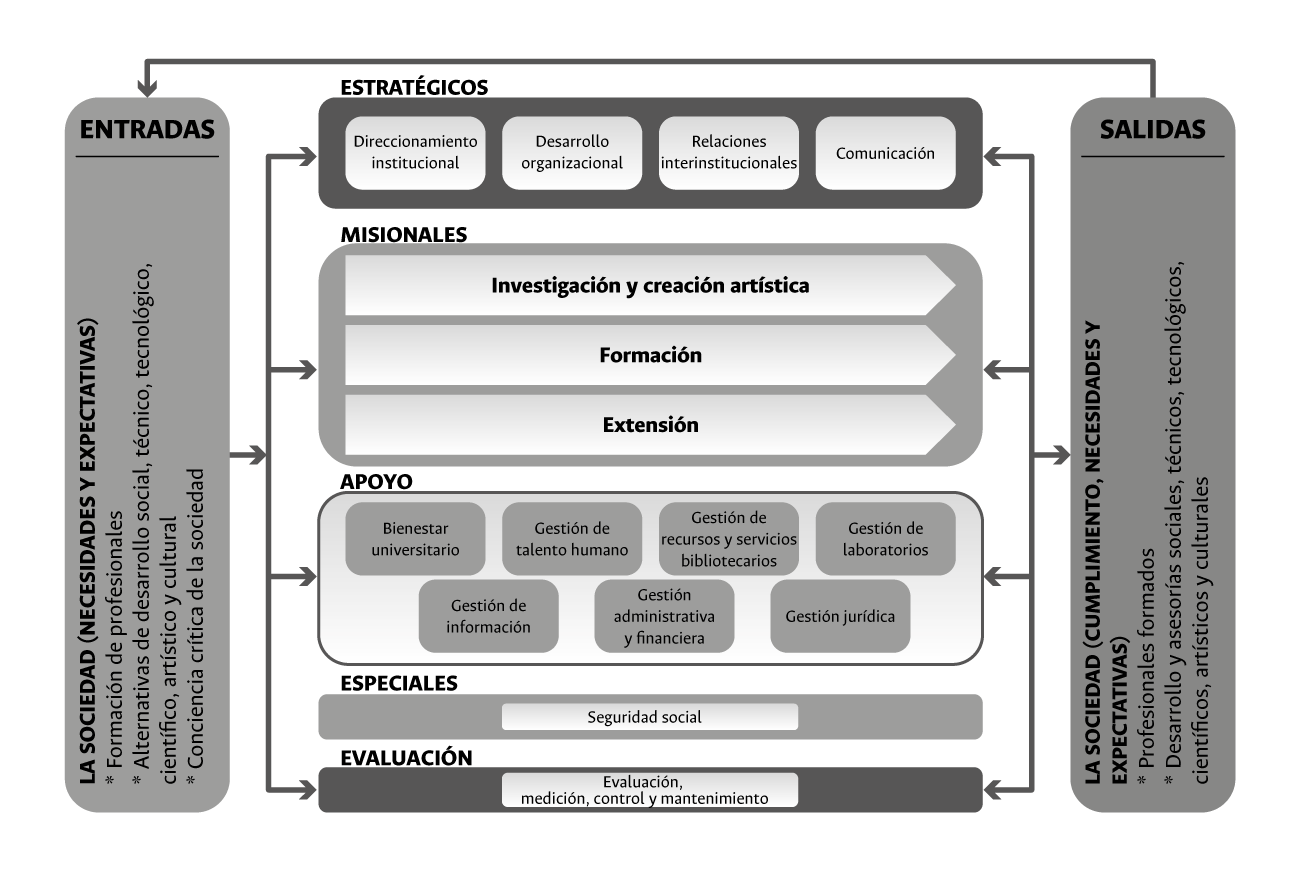
\includegraphics[width=0.8\linewidth]{Imagenes/F_2} 

}

\caption{Mapa de procesos institucionales. Tomado de Gestión por procesos en http://siga.unal.edu.co/index.php/procesos/gestion-por-procesos1.}\label{fig:fig2}
\end{figure}

\hypertarget{medicion}{%
\chapter{Seguimiento y medición}\label{medicion}}

Seguimiento, medición, análisis y evaluación

\hypertarget{alcance}{%
\section{Alcance}\label{alcance}}

\hypertarget{medidas}{%
\chapter{Tipos de medidas}\label{medidas}}

Existen tres tipos de medidas

\hypertarget{estadisticas}{%
\section{Estadísticas}\label{estadisticas}}

Como lo presenta \citet{Alberto2019}, las estadísticas\footnote{Nombre
  que se emplea para diferenciarlo de \ldots{}}

\hypertarget{indicadores-estadisticos}{%
\section{Indicadores estadísticos}\label{indicadores-estadisticos}}

\hypertarget{indicadores-de-cumplimiento}{%
\section{Indicadores de
cumplimiento}\label{indicadores-de-cumplimiento}}

\hypertarget{indicadoresUN}{%
\chapter{Medición de los procesos en la UN}\label{indicadoresUN}}

\hypertarget{principios}{%
\section{Principios}\label{principios}}

\hypertarget{gobernabilidad}{%
\section{Gobernabilidad}\label{gobernabilidad}}

\hypertarget{un-proceso-especial}{%
\section{Un proceso especial}\label{un-proceso-especial}}

\hypertarget{anexos}{%
\chapter*{Anexos}\label{anexos}}
\addcontentsline{toc}{chapter}{Anexos}

\bibliography{book.bib,packages.bib}


\end{document}
